\subsection{Beschaffung von der Hotelart}
\label{subsubsec:hotelart}
Einer der wichtigsten Eigenschaften, die ein Hotel vorweisen kann, ist die Hotelart von dem jeweiligen Hotel. Die Hotelart hängt maßgeblich mit der zur grundlegenden Preisgestaltung ab. Dies ist einfach zu erklären, da Hotels existieren, die eher auf Wellness ausgelegt sind und somit prinzipiell teurer sind als einfache Urlaubshotels. Somit ist die Art eines Hotels essentiell, um ähnliche Hotels zu finden. So soll auch für das Modell die Hotelart vorhanden sein. Dieses Feature muss jedoch erst beschafft werden, da diese Information nicht in der Datenbank hinterlegt ist. 
\newline
\newline
Leider ist der Versuch, die Hotelart auf einem automatisiertem Weg zu bekommen, gescheitert, und es blieb nichts anderes übrig, als die Hotelart eines jeden Hotels manuell herauszufinden. 
\newline
\newline
Nachdem die Hotelart beschaffen wurde, sieht der Feature-Datensatz wie folgt aus:
\begin{figure}[h]
    \centering
    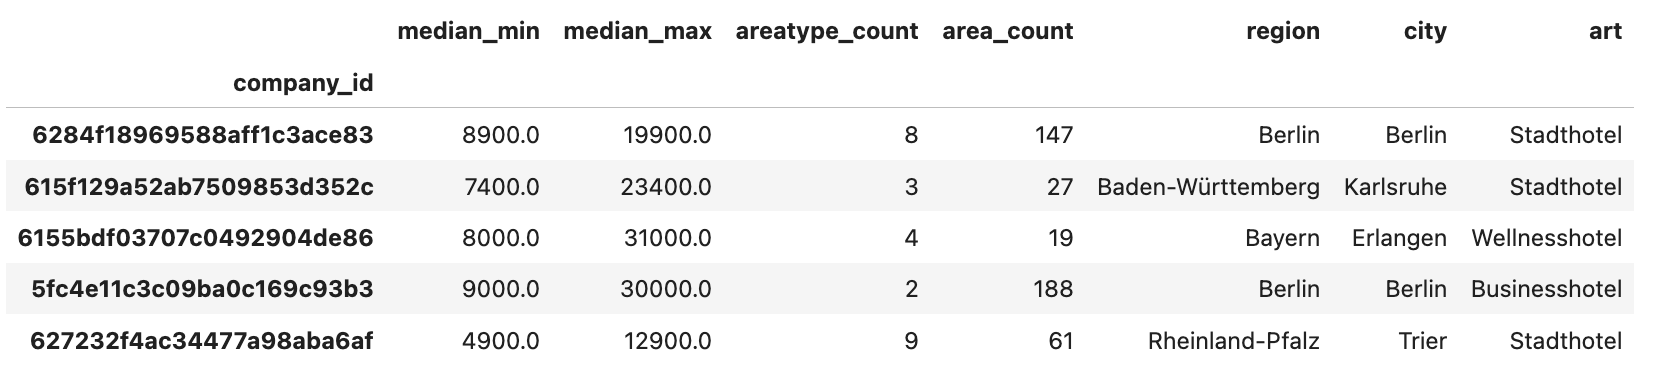
\includegraphics[width=1\textwidth, center]{Features_2.png}
    \caption[Alle schon vorhanden Features #2]{Alle schon vorhanden Features #2}
    \label{img:all_Features_2}
\end{figure}
